%%%%%%%%%%%%%%%%%%%%%%%%%%%%%%%%%%%%%%%%%
% Short Sectioned Assignment
% LaTeX Template
% Version 1.0 (5/5/12)
%
% This template has been downloaded from:
% http://www.LaTeXTemplates.com
%
% Original author:
% Frits Wenneker (http://www.howtotex.com)
%
% License:
% CC BY-NC-SA 3.0 (http://creativecommons.org/licenses/by-nc-sa/3.0/)
%
%%%%%%%%%%%%%%%%%%%%%%%%%%%%%%%%%%%%%%%%%

%----------------------------------------------------------------------------------------
%	PACKAGES AND OTHER DOCUMENT CONFIGURATIONS
%----------------------------------------------------------------------------------------

\documentclass[paper=a4, fontsize=11pt]{scrartcl} % A4 paper and 11pt font size
\usepackage[top=2.5cm, bottom=2.5cm, left=2.5cm, right=2cm]{geometry}
\usepackage[normalem]{ulem}
\usepackage[T1]{fontenc} % Use 8-bit encoding that has 256 glyphs
\usepackage{fourier} % Use the Adobe Utopia font for the document - comment this line to return to the LaTeX default
\usepackage[english]{babel} % English language/hyphenation
\usepackage{amsmath,amsfonts,amsthm} % Math packages

\usepackage{sidecap}
\usepackage{hyperref}
\hypersetup{colorlinks,urlcolor=blue}

\usepackage{listings}
\lstset{language=BASH}
\usepackage{xcolor}
\usepackage{graphicx}
\graphicspath{ {./images/} }
\usepackage[toc,page]{appendix}

\usepackage{color}

\definecolor{mygreen}{rgb}{0,0.6,0}
\definecolor{mygray}{rgb}{0.5,0.5,0.5}
\definecolor{mymauve}{rgb}{0.58,0,0.82}
\definecolor{light-gray}{gray}{0.95}

\lstset{ %
  backgroundcolor=\color{light-gray},   % choose the background color; you must add \usepackage{color} or \usepackage{xcolor}
  basicstyle=\footnotesize,        % the size of the fonts that are used for the code
  breakatwhitespace=false,         % sets if automatic breaks should only happen at whitespace
  breaklines=true,                 % sets automatic line breaking
  captionpos=b,                    % sets the caption-position to bottom
  commentstyle=\color{mygreen},    % comment style
  deletekeywords={...},            % if you want to delete keywords from the given language
  escapeinside={\%*}{*)},          % if you want to add LaTeX within your code
  extendedchars=true,              % lets you use non-ASCII characters; for 8-bits encodings only, does not work with UTF-8
  frame=single,	                   % adds a frame around the code
  keepspaces=true,                 % keeps spaces in text, useful for keeping indentation of code (possibly needs columns=flexible)
  keywordstyle=\color{purple},       % keyword style
  language=bash,                 % the language of the code
  otherkeywords={*,emacs,sudo, tkmedit, recon-all, freeview, ls, recon-all-go, ship-data, mv, cp, date, touch, FS-stats, FSQC-check, FSQC-makehtml, FSQC-summary, nextract.batch, nextractomatic, git, clone},           % if you want to add more keywords to the set
  numbers=none,                    % where to put the line-numbers; possible values are (none, left, right)
  numbersep=5pt,                   % how far the line-numbers are from the code
  numberstyle=\tiny\color{mygray}, % the style that is used for the line-numbers
  rulecolor=\color{black},         % if not set, the frame-color may be changed on line-breaks within not-black text (e.g. comments (green here))
  showspaces=false,                % show spaces everywhere adding particular underscores; it overrides 'showstringspaces'
  showstringspaces=false,          % underline spaces within strings only
  showtabs=false,                  % show tabs within strings adding particular underscores
  stepnumber=2,                    % the step between two line-numbers. If it's 1, each line will be numbered
  stringstyle=\color{mymauve},     % string literal style
  tabsize=2,	                   % sets default tabsize to 2 spaces
  title=\lstname                   % show the filename of files included with \lstinputlisting; also try caption instead of title
}

\usepackage{sectsty} % Allows customizing section commands
\allsectionsfont{\centering \normalfont\scshape} % Make all sections centered, the default font and small caps
\makeatletter
\g@addto@macro\@floatboxreset\centering
\makeatother

\usepackage{fancyhdr} % Custom headers and footers
\pagestyle{fancyplain} % Makes all pages in the document conform to the custom headers and footers
\fancyhead{} % No page header - if you want one, create it in the same way as the footers below
\fancyfoot[L]{} % Empty left footer
\fancyfoot[C]{} % Empty center footer
\fancyfoot[R]{\thepage} % Page numbering for right footer
\renewcommand{\headrulewidth}{0pt} % Remove header underlines
\renewcommand{\footrulewidth}{0pt} % Remove footer underlines
\setlength{\headheight}{13.6pt} % Customize the height of the header

\numberwithin{equation}{section} % Number equations within sections (i.e. 1.1, 1.2, 2.1, 2.2 instead of 1, 2, 3, 4)
\numberwithin{figure}{section} % Number figures within sections (i.e. 1.1, 1.2, 2.1, 2.2 instead of 1, 2, 3, 4)
\numberwithin{table}{section} % Number tables within sections (i.e. 1.1, 1.2, 2.1, 2.2 instead of 1, 2, 3, 4)



%----------------------------------------------------------------------------------------
%	TITLE SECTION
%----------------------------------------------------------------------------------------

\newcommand{\horrule}[1]{\rule{\linewidth}{#1}} % Create horizontal rule command with 1 argument of height

\title{	
\normalfont \normalsize 
\textsc{Center for Functional \& Molecular Imaging \\ Georgetown University Medical Center} \\ [25pt] % Your university, school and/or department name(s)
\horrule{0.5pt} \\[0.4cm] % Thin top horizontal rule
\huge Brain Morphometry Analyses in FreeSurfer I:  Reconstructing Structural MRI Scans  \\ % The assignment title
\horrule{2pt} \\[0.5cm] % Thick bottom horizontal rule
}

\author{Made for CFMI training} % Your name

\date{\normalsize 4 November 2015} % Today's date or a custom date

\begin{document}

\maketitle % Print the title

\lstset{escapechar=\@} % escape lstlisting
%----------------------------------------------------------------------------------------
% INTRO
\section{Introduction}  \href{https://surfer.nmr.mgh.harvard.edu/}{Freesurfer} (FS) is a powerful (and freely available!) software package developed at the Martinos Center for Biomedical Imaging for automatized analyses of brain anatomy.  A non-inclusive list of its capabilities includes:
\begin{itemize}
	\item Performing morphometric analysis of the brain \\  \textit{(i.e. cortical thickness, curvature, surface area, volume)}
	\item Creating study-specific anatomical templates
	\item Optimal alignment of cortical folding patterns across individuals
	\item Processing of functional imaging data using the FSFAST software suite
	\item Segmenting and aligning individual brain volumes to an anatomical atlas
	\item Rendering 3D models of the pial surface, white-matter and user-defined masks
\end{itemize}

Although FS possesses remarkable capabilities that greatly reduce the effort involved in analyzing structural MRI data, there are crucial caveats the user must be aware of. This document is the first in a series of training guides intended to bring a novice user up to speed on using and trouble-shooting FS.  In this guide, we will describe how to install and configure your system for FS and then walk you through the steps of reconstructing a brain scan from raw data and viewing the final results.  Part II in this series, "Trouble Shooting \& Manual Editing" will outline steps for artifact correction and manual intervention at various steps along the FS anatomical analysis workflow. Part III will cover statistical methods for morphometric analyses.

The materials presented here are collected from miscellaneous notes taken from the \href{https://surfer.nmr.mgh.harvard.edu/fswiki}{FreeSurfer Wiki}, \href{http://www.mail-archive.com/freesurfer@nmr.mgh.harvard.edu/}{list-serv user postings}, \href{https://www.zotero.org/freesurfer}{published papers} and independent experimentation.  If a question comes up that is not addressed in this guide be sure to consult these resources first! If all else fails, ask questions! \mbox{\textit{(Also see Appendix)}}
%%
% BACKGROUND
\subsection{Background}
\paragraph{Cortical Surface Reconstruction} FS initially emerged from efforts to constrain the \href{http://www.scholarpedia.org/article/Source_localization}{inverse problem for EEG/MEG source localization} using anatomically accurate cortical surface models \cite{dale_improved_1993}.  Dale \& Sereno's major innovation was to use the gray/white boundary instead of the pial surface to reconstruct the cortex -- effectively curtailing the challenge of conforming a continuous spherical surface to a highly irregular and non-continuous cortical surface.  However, these early attempts did not produce accurate surface models and required extensive user intervention to correct topological defects. The accuracy of surface deformation techniques is constrained by three considerations:
\begin{enumerate}
\item \textbf{Iso-Intensity Surfaces} -- the assumption that the MRI intensity of gray/white and pial surfaces are constant. However, this assumption is not accurate. Cortical tissue varies in micro anatomy and thus the signal intensity is quite variable across cortex.  For example, myelin-rich regions will appear much brighter than myelin-poor regions.
\item \textbf{Topological Constraints} -- surfaces must be constrained to not self intersect.  This problem is made exceptionally difficult since the cortex is tightly packed making the demarcation between adjacent sulcal banks a hard computational problem for planar Eulerian methods.
\item \textbf{Curvature minimization} -- smooth surfaces are generated through curvature minimization, however cortex contains many regions with high curvature.
\end{enumerate}

Fischl \& Dale addressed concern \#1 by adaptively determining MR intensity thresholds for a boundary at each point in an image, concern \#2 by avoiding curvature minimization and using a second-order polynomial patch instead of a plane surface and concern \#3 by applying fast triangle-triangle intersection borrowed from the computer graphics literature \cite{fischl_measuring_2000}.  This method proved to produce accurate and sensitive \mbox{(up to $\frac{1}{4}$ mm)} measurements of cortical thickness that withstood considerable variation in sequence parameters, acquisition artifacts and tissue variability \cite{fischl_automated_2001}.  Many groups have now validated Fischl \& Dale's reconstruction algorithm with histological and manual measures across many scanner platforms, in the presence of subject motion, different acquisition parameters, correlations with behavioral measures and analysis types \cite{dickerson_detection_2008,  han_reliability_2006, rosas_regional_2002, ReutEtal14, vonEconomo}.  

\paragraph{Whole Brain Segmentation} Once the cortical surface reconstruction approach had been tackled, Fischl et al. turned their attention to whole brain segmentation.  The major difficulty in performing algorithmic volumetric segmentation of the gray matter is the high variability of image intensity across brain structures. A Bayesian approach was adopted to solve this problem using a  different model to compute the image likelihood at each position in space. A non-stationary, anistrophic Markov Random Field model was used to define the prior on structure identity given relative spatial location to other macro-structures. The technique was validated using a training set of manually labeled images, achieving comparable performance to extensively trained personnel and exhibited excellent performance with pathological samples \cite{fischl_whole_2002, fischl_sequence-independent_2004}.

\paragraph{Other Contributions}
Many other groups have contributed improvements and additional modules to the FS software suite: 
 \begin{itemize}
\item Tractography \cite{yendiki_automated_2011}
\item Alignment of Cortical Folding Patterns and Subcortical/Ventricular Structures
\cite{postelnicu_combined_2009}
\item Analysis of Cortical Curvature Development \cite{pienaar_methodology_2008}
\item Skull Stripping \cite{segonne_hybrid_2004}
\item Statistical Models for Longitudinal Analyses \cite{reuter_within-subject_2012}
\item Gyral Based Cortical Parcellation \cite{desikan_automated_2006}
\item Insensitivity to Pulse Sequences \cite{han_reliability_2006}
\item High Resolution Segmentation of Hippocampal Subfields \cite{van_leemput_automated_2009}
\item Probabilistic Label Segmentation \cite{sabuncu_generative_2010}
\end{itemize}


Thanks to the efforts of those that validated and built-upon the software, cognitive neuroscientists and clinicians can accurately measure a variety of morphometrics in relation to brain function. Now that you are stoked after perusing this exciting scientific historical backdrop, continue on to learn how to install FS and run your first cortical reconstruction.
%------------------------------------------------
% INSTALLATION
\section{Installation \& System Configuration}
The following installation instructions are tailored to OS X/Linux users with some familiarity of command line usage.  Please see the FS instructions if you are an unfortunate Microsoft user. Procedural hints for these instructions are included in the Appendix.  If anything is confusing at all don't hesitate to ask!
\begin{enumerate}
\item \href{ftp://surfer.nmr.mgh.harvard.edu/pub/dist/freesurfer/5.3.0/freesurfer-Darwin-lion-stable-pub-v5.3.0.dmg}{Download FreeSurfer}
\item Add the FS start-up routine to your \texttt{.bash\_profile.}  To do this open a terminal, cd into your home directory and open \texttt{.bash\_profile} in a text editing program such as emacs, vi or nano
\begin{lstlisting}[frame=single]
cd ~
emacs .bash_profile
\end{lstlisting}
Edit your .bash\_profile to include the commands below.  Make sure the  \href{https://en.wikipedia.org/wiki/Shebang_(Unix)}{she-bang} (\texttt{\#!/bin/bash} ) is included at the top if you are creating the file from scratch.  This tells your terminal what program is used to run these commands.  
\begin{lstlisting}[frame=single]
#!/bin/bash
# FREESURFER SETUP
export FREESURFER_HOME="/Applications/freesurfer"
source $FREESURFER_HOME/SetUpFreeSurfer.sh
export SUBJECTS_DIR="/Applications/freesurfer/subjects"
\end{lstlisting}
After verifying everything looks ok, type the \texttt{control} key then \texttt{x}, the \texttt{control} key again, then \texttt{c} to exit and save (for emacs). You will be prompted whether you want to save the file before exiting.  Type \texttt{y} then hit \texttt{enter} to do so. 
\\~ \\~
The commands you added to your \texttt{.bash\_profile} put the FS tools at your disposal each time you open a terminal window.  Note that you may eventually want to change your \texttt{SUBJECTS\_DIR} to the path of your own data directory:
\begin{lstlisting}[frame=single]
SUBJECTS_DIR="/exports/home/<cfmiuser>/ADS/ads.subjects"
\end{lstlisting}
\item Next open up the \texttt{.dmg} file you downloaded in step 1 and go through the installer.
\item Then register on the FS website to get a \href{https://surfer.nmr.mgh.harvard.edu/registration.html}{license}.
\\~ \\~
\item When it is emailed to you, use \texttt{emacs} to create a license file then copy and paste in the key. You will need an administrator password for this since you must use super-user do:
\begin{lstlisting}[frame=single]
sudo emacs /Applications/freesurfer/.license
\end{lstlisting}  

\item IMPORTANT: be sure to source your \texttt{.bash\_profile} so you can use FS at the terminal
\begin{lstlisting}[frame=single]
cd ~
. .bash_profile
\end{lstlisting}
\item Run your first test of the installation by typing the following into a terminal
\begin{lstlisting}[frame=single]
tkmedit $FREESURFER_HOME/subjects/bert orig.mgz
\end{lstlisting}
\end{enumerate}

%------------------------------------------------
% RECON ALL QUICK START
\section{Reconstruct them all!}
\subsection{Quick-Start Tutorial} The most attractive feature of  FS is that it makes cortical surface reconstruction and subcortical segmentation for a single subject as easy as typing in a single command and coming back the next day to check your results.  To get started, you must set up your environment and import your imaging data.
\paragraph{Environment Setup}You may clone a repository containing all of the tools you will require for this tutorial by typing the following into a terminal window

\begin{lstlisting}
cd ~
git clone https://@git@hub.com/seldamat/Surfer-gems.@git
\end{lstlisting}

~\\The \texttt{ls} command can be used to view the contents of this repository

\begin{lstlisting}
ls ~/Surfer-gems
@FS-stats @
@FSQC-check@
@FSQC-makehtml@
@FSQC-summary@
@README.md@
@doc@
@nextract.batch@
@nextractomatic@
@recon-all-go@
@ship-data@
\end{lstlisting}

~\\General information about the repository can be found within the \texttt{README} file.  The \texttt{doc} directory contains the \LaTeX\  files used to generate this document.  Note that this repository is updated frequently.  The \href{http://rogerdudler.github.io/git-guide/}{git command line tool} can keep you up to date with the newest versions.

~\\Usage information about any of the programs can be obtained by calling the program by name with an appended \texttt{-h} option.  For example,

\begin{lstlisting}
cd ~/Surfer-gems
ship-data -h

@ship-data@ - A wrapper @for@ the rsync @function@ to quickly sync large data directories.

	Usage   :: @ship-data@ DATASOURCE DESTINATIONFOLDER

	Example :: @ship-data@ ~/mydata ~/projectfolder

	Extra Info ::

		!! the datasource will be placed inside the project folder

		!! If the project folder contains a directory with the same
	   	name as the data @source@, @then@ the folder will not be
	   	overwritten but rater up@date@d.  Only newer files will be
	   	kept.  Older files are overwritten.

		!! Do not use slashes at the end of directory paths

		!! sync information is written to shipping.log, a file
		located @in@ the project folder
\end{lstlisting}

\paragraph{Importing Raw Data} At the CFMI, the original \texttt{.IMA} DICOM files are usually downloaded or copied from the raw data directory on the server and converted to \texttt{.nii} or \texttt{.img/.hdr}.  A program for performing automatic conversion and data duplication can be found at \mbox{\texttt{\textasciitilde/Surfer-gems/nextractomatic}}.   This program uses the \texttt{dcm2niix} conversion software and is written specifically to handle the CFMI mySQL database. Software such as \href{http://neuro.debian.net/pkgs/mriconvert.html}{MRICONVERT} or \href{http://www.mccauslandcenter.sc.edu/mricro/mricron/}{MRICRON} may also be used for this purpose.  An example call of \texttt{nextractomatic} appears below

\begin{lstlisting}
nextractomatic \
		-r /exports/home/se394/ADS/data/raw/w1 \	# Path to raw dicom .IMA data
		-s "149959" \															# Subject ID
		-dm 2012-6-14 -dx 2012-6-15 \							# Date range of scans to extract
		-rf .nii \																# Conversion format
		-t "MPRAGE Rest" \ 												# Scan names to extract
		-ra "Anat Rest"													# New names for scans
\end{lstlisting}

~\\Sometimes pre-existing data may have already been converted and stored in a central project directory on the server.  If this is the case, it is more efficient to copy the data over to your own local user project directory, perform your analyses then ship the data back to the central project directory.  To accomplish this, you can use the \texttt{ship-data} program found within the \texttt{Surfer-gems} repository.

~\\ \\ Once the environment for FS has been set, you are ready to analyze your first subject.  First you must import the raw image files to your \texttt{SUBJECTS\_DIR} by typing the following into a terminal:
\begin{lstlisting}[frame=single, xrightmargin=0cm]
recon-all -s <subjectname> -i <pathtorawdata1.nii> \
			                     -i <pathtorawdata2.nii>
\end{lstlisting}

~\\The \texttt{-i} option copies the raw image files after they have been converted to \texttt{NIFTI} to the directory structure required for running the \texttt{recon-all} command.  Multiple input images can be specified if more than one run exists for a given subject.  These runs are averaged together to generate cleaner images.

~\\After importing your data to the FreeSurfer directory structure, take a look in \texttt{SUBJECTS\_DIR} and you should see a folder for the subject with the following directories:
\begin{lstlisting}[frame=single]
ls $SUBJECTS_DIR/<subjectname>
bem
label
mri
scripts
src
stats
surf
temp
@touch@
trash
\end{lstlisting}
We will explain the purpose of some of these folders later.  For now, you can view the original raw mri
\begin{lstlisting}[frame=single]
tkmedit <subjectname> orig/001.mgz
\end{lstlisting}
~\\
Once it is confirmed that the subject has been successfully imported, we can begin the processing stream
\begin{lstlisting}[frame=single]
recon-all -s <subjectname> -all
\end{lstlisting}

The pre-processing can take up to 24 or as little as 4 hours depending on your machine.  Optimizing this work flow is absolutely crucial when performing a large study with many subjects.
%------------------------------------------------
% BATCH PROCESSING
\subsection{Batch Processing}
Batches of subjects can be run by writing bash scripts to loop across a list of subjects, invoking recon-all for each one.  As previously mentioned, each individual subject can take up to 24 hours to complete reconstruction thus it is highly desirable to run your batches in parallel across as many nodes as possible.  A user can run as many recon-all sessions on a single system as there are processor cores or nodes on that system.  
\paragraph{LockFiles \& Adaptive Iteration} One way to make parallel FS processing more efficient is to prevent different instances of \texttt{recon-all} from processing the same subject by using a lock-file.  The lock-file is a temporary file that is created as a particular subject is currently being processed so that any new invocations of \texttt{recon-all} know to move on to the next unprocessed subject.  

The problem becomes much more complicated when multiple users are running \texttt{recon-all} with large subject databases hosted on a server.  In this instance, we avoid re-processing already completed subjects  by cross-checking each \texttt{recon-all} call with a list of completed subjects. In conjunction with a lock-file, this prevents different users from processing or re-processing the same subject.

These considerations are implemented in the batch processing script \href{https://www.dropbox.com/s/j7zmp29bkdeg9h5/recon-all-go.sh?dl=0}{\texttt{recon-all-go.sh}}.  This script requires a project directory, subjects directory, list of subjects, and subject wave as input.  The subject wave is null,'', by default (i.e. if not provided). For example:

\begin{lstlisting}
. recon-all-go -pd /exports/home/<cfmiuser>/Projects/ADS/ -s analysis.1.subject.list
\end{lstlisting}

Be sure to only include the subjects you would like to process in the raw data directory because the script processes the entire contents of that folder. Note that the name of each scan \textit{must} begin with \texttt{'Anat'} followed by a wildcard (\texttt{*}) and a \texttt{.img} file extension. If a subject list file does not already exist, then the script will create it with the \texttt{-s} input using all subjects under \texttt{./data/Subjects/\$subwave}. Note again that by default \texttt{\$subwave=''}. This means the script assumes every subdirectory under 
\\ \texttt{./data/Subjects/} is a subject directory.  Indicate which subdirectory your subject data lives in using the \texttt{-w} flag. Lastly, make sure to copy the source data directory to your local home folder first before beginning analyses.  i.e)
\begin{lstlisting}
. ship-data.sh -s /exports/processed/data/ADS/Subjects/Wave1 -ss Anat \
																	-target ~/Projects/ADS/data/Subjects/Wave1
\end{lstlisting}
%------------------------------------------------
% VIEWING RESULTS
\section{Perusing the Results}  FS comes with multiple image visualization programs for editing, viewing and overlaying anatomical/functional brain scans.  \texttt{Tksurfer} and \texttt{Tkmedit} are older, C-based legacy programs whereas \texttt{Freeview} is much newer and has a great ergonomic design.  We will cover how to use \texttt{Freeview} to inspect your first recon-all results. To view a subject's T1, white matter mask, brain mask subcortical segmentation and surface reconstruction in \texttt{Freeview}, open a terminal and type:
\begin{lstlisting}[frame=single]
subjid=<subjectid>
SUBJECTS_DIR="/exports/home/<cfmiuser>/ADS/Projects/data/ads.subjects.tutorial"
alias launchfv="freeview -v $SUBJECTS_DIR/$subjid/mri/brainmask.mgz \                                                                               
$SUBJECTS_DIR/$subjid/mri/aseg.mgz:colormap=lut:opacity=0.2\                                                                                        
$SUBJECTS_DIR/$subjid/mri/T1.mgz \                                                                                                                  
$SUBJECTS_DIR/$subjid/mri/wm.mgz:colormap=heat:opacity=0.4:visible=0 \                                                                              
-f $SUBJECTS_DIR/$subjid/surf/lh.white:edgecolor=blue \                                                                                             
$SUBJECTS_DIR/$subjid/surf/lh.pial:edgecolor=red \                                                                                                  
$SUBJECTS_DIR/$subjid/surf/rh.white:edgecolor=blue \                                                                                                
$SUBJECTS_DIR/$subjid/surf/rh.pial:edgecolor=red \                                                                                                  
$SUBJECTS_DIR/$subjid/surf/lh.smoothwm.nofix:visible=0 \                                                                                            
$SUBJECTS_DIR/$subjid/surf/rh.smoothwm.nofix:visible=0 \                                                                                            
$SUBJECTS_DIR/$subjid/surf/lh.inflated:visible=0 \                                                                                                  
$SUBJECTS_DIR/$subjid/surf/rh.inflated:visible=0"
\end{lstlisting}
The \texttt{-v} flag is used to open volume data and the \texttt{-f} flag is used to load surfaces.  You can indicate which colormap, color, opacity and other plotting options by indicating them with a colon following the file name.  We can create an alias, or a shortcut, to avoid typing this very long command every time you want to visualize a new subject.   To define an alias, open your \texttt{.bash\_profile} and include the following commands.

\begin{lstlisting}
export SUBJECTS_DIR="/exports/home/<cfmiuser>/ADS/Projects/data/ads.subjects.tutorial"
alias launchfv="freeview -v $SUBJECTS_DIR/$subjid/mri/brainmask.mgz \                                                                               
$SUBJECTS_DIR/$subjid/mri/aseg.mgz:colormap=lut:opacity=0.2\                                                                                        
$SUBJECTS_DIR/$subjid/mri/T1.mgz \                                                                                                                  
$SUBJECTS_DIR/$subjid/mri/wm.mgz:colormap=heat:opacity=0.4:visible=0 \                                                                              
-f $SUBJECTS_DIR/$subjid/surf/lh.white:edgecolor=blue \                                                                                             
$SUBJECTS_DIR/$subjid/surf/lh.pial:edgecolor=red \                                                                                                  
$SUBJECTS_DIR/$subjid/surf/rh.white:edgecolor=blue \                                                                                                
$SUBJECTS_DIR/$subjid/surf/rh.pial:edgecolor=red \                                                                                                  
$SUBJECTS_DIR/$subjid/surf/lh.smoothwm.nofix:visible=0 \                                                                                            
$SUBJECTS_DIR/$subjid/surf/rh.smoothwm.nofix:visible=0 \                                                                                            
$SUBJECTS_DIR/$subjid/surf/lh.inflated:visible=0 \                                                                                                  
$SUBJECTS_DIR/$subjid/surf/rh.inflated:visible=0"
\end{lstlisting}

The alias can be invoked from a terminal after you source your \texttt{.bash\_profile}.  Note that you must define your subjects directory, \texttt{\$SUBJECTS\_DIR}, and the specific subject, \texttt{\$subjid}, you want to see. Once you add the alias, you may use it like-so:

\begin{lstlisting}
subjid="149959"
. .bash_profile #source the new commands, do this for every new subjid definition
launchfv
\end{lstlisting}

Freeview gives you many options to view and manipulate your subject's processed results. To learn more about the Freeview graphical interface and key-mappings to functions please read this \href{https://surfer.nmr.mgh.harvard.edu/fswiki/FsTutorial/OutputData_freeview}{tutorial}.
%------------------------------------------------
% UNDER THE HOOD
\section{Under-the-hood}
\begin{figure}[h]
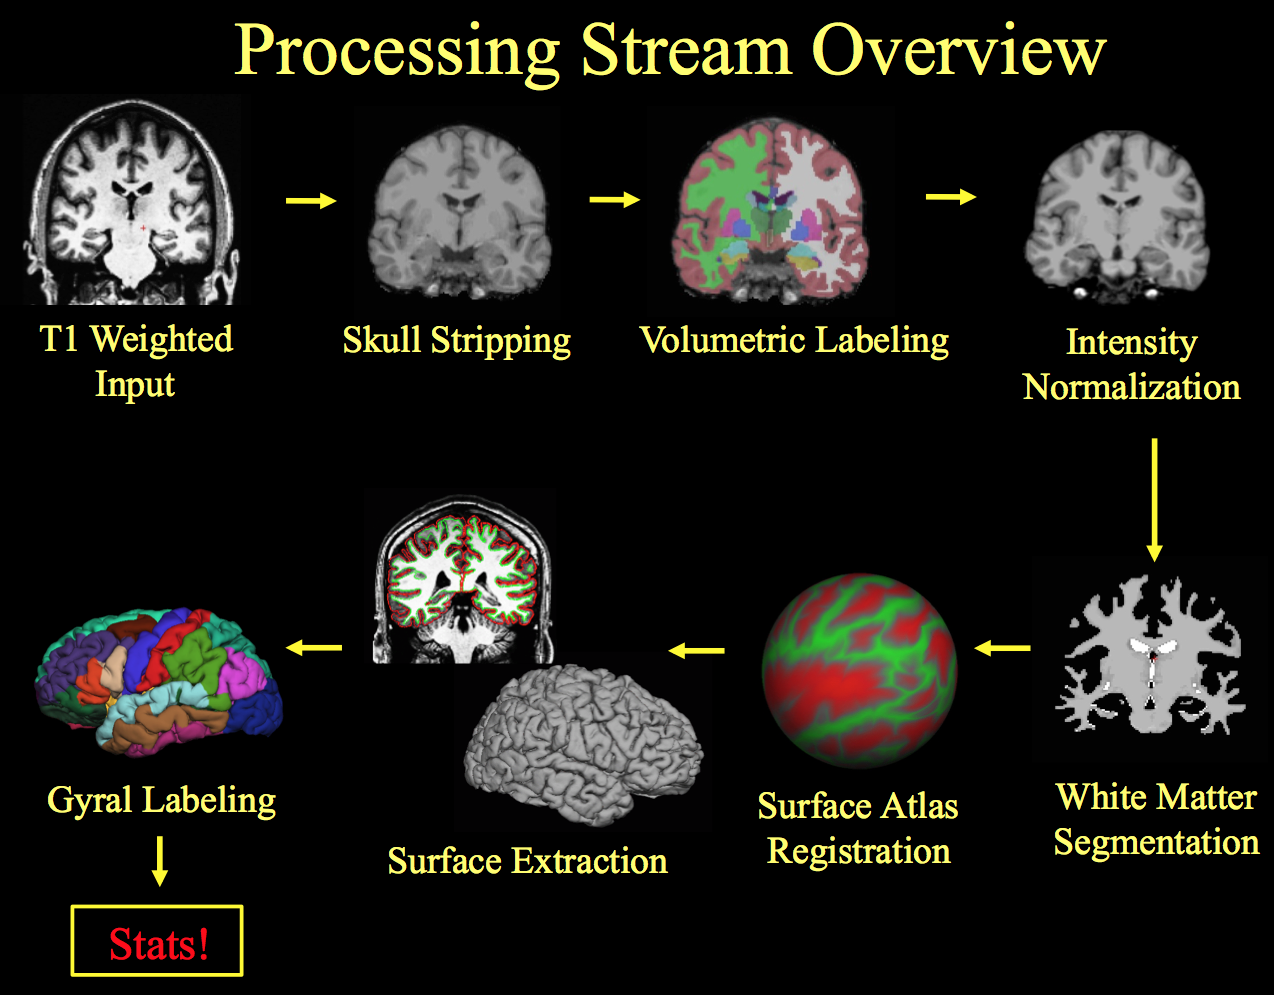
\includegraphics[width=13cm,height=10cm]{FSprocstream}
\caption{\textbf{FS Processing Stream}}
\end{figure}
While you are running your first subject you may notice that the terminal will quickly begin filling up with text describing the processing status, any errors that may have been encountered and details regarding individuals steps taken.  You can get more information about each of these steps and the usage of recon-all by opening a new terminal and typing:
\begin{lstlisting}[frame=single]
recon-all -help
\end{lstlisting}
The help command also provides you with information regarding optional arguments you can flag each recon-all call with.  Of particular importance are the autorecon flags:
\begin{lstlisting}
-autorecon1  :  process stages 1-5
-autorecon2  :  process stages 6-23
-autorecon3  :  process stages 24-34
\end{lstlisting}
Each of these flags can take additional options for algorithm parameters or to only run a subset of the processing stages. The individual stages and some optional parameters of the FS pre-processing pipeline are summarized below.
%% AUTORECON PROCESSING STAGES
%% -- ADD FIGURES AT ONE POINT OR ANOTHER
\paragraph{Autorecon consists of 34 processing stages:}
\begin{enumerate}
    \item  \textbf{Motion Correction and Conform} -- Multiple scans from the same subject are averaged together to minimize motion artifacts.  The input are the volumes found in file(s) \texttt{mri/orig/XXX.mgz}. The output will be the volume \texttt{mri/orig.mgz}. If no runs are found, then it looks for a volume in \texttt{mri/orig}. If that volume is there, then it is used in subsequent processes as if it was the motion corrected volume. If no volume is found, then the process exits with errors.
    
    \item  \textbf{NU (Non-Uniform intensity normalization) }-- Non-parametric Non-uniform intensity Normalization (N3), corrects for intensity non-uniformity in MR data, making relatively few assumptions about the data. This runs the MINC tool \texttt{nu\_correct}. By default, four iterations of \texttt{nu\_correct} are run. The flag \texttt{-nuiterations} specification of some other number of iterations.
    
    \item  \textbf{Talairach transform computation} -- The affine matrix required to register the scan to the MNI305 space is computed at this step.  You can/should check the talairach registration using \texttt{tkregister2 --s subjid --fstal}. \texttt{tkregister2} allows you to compare the original volume against the talairach volume resampled into the original space. Run \texttt{tkregister2 --help} for more information. This step creates the files \texttt{mri/transform/talairach.auto.xfm} and \texttt{talairach.xfm}.
    
    \item  \textbf{Intensity Normalization 1}  -- Renormalization of intensity. Performs intensity normalization of the \texttt{orig} volume and places the result in \texttt{mri/T1.mgz}. Attempts to correct for fluctuations in intensity that would otherwise make intensity-based segmentation much more difficult. \textit{Intensities for all voxels are scaled so that the mean intensity of the white matter is 110.} If there are problems with the normalization, users can add control points. (See part II for more info) 
    
    \item  \textbf{Skull Strip} -- The skull and brainstem are removed from \texttt{mri/T1.mgz} and stores the result in \\ \texttt{mri/brainmask.auto.mgz} and \texttt{mri/brainmask.mgz}. Runs the \texttt{mri\_watershed} program. \textit{If the strip fails, users can specify seed points} (\texttt{-wsseed}) \textit{or change the threshold} (\texttt{-wsthresh, -wsmore, -wsless}). The \texttt{-autorecon1} stage ends here.
    
    \item  \textbf{EM Register (linear volumetric registration)} -- Computes transform to align the \texttt{mri/nu.mgz} volume to the default GCA atlas found in \texttt{\$FREESURFER\_HOME/average} (see \texttt{-gca} flag for more info). Creates the file \texttt{mri/transforms/talairach.lta}. The \texttt{-autorecon2} stage starts here.
    
    \item  \textbf{CA Intensity Normalization} -- Further normalization, based on GCA model. Creates \texttt{mri/norm.mgz}.

    \item  \textbf{CA Non-linear Volumetric Registration } --Computes a nonlinear transform to align with GCA atlas. Creates the file \texttt{mri/transform/talairach.m3z}.
    
    \item  \textbf{Remove neck} -- The neck region is removed from the NU-corrected volume \texttt{mri/nu.mgz}. Makes use of transform computed from prior CA Register stage. Creates the file \texttt{mri/nu\_noneck.mgz}.
    
    \item \textbf{EM Register, with skull} --Computes transform to align volume \texttt{mri/nu\_noneck.mgz} with GCA volume possessing the skull. Creates \texttt{mri/transforms/talairach\_with\_skull.lta}.
    
    \item \textbf{CA Label (Aseg: Volumetric Labeling) and Statistics} -- Labels subcortical structures, based in GCA model. Creates the files \texttt{mri/aseg.auto.mgz} and \texttt{mri/aseg.mgz}.
    \item \textbf{Intensity Normalization 2 (start here for control points)} -- Performs a second (major) intensity correction using only the brain volume as the input (so that it has to be done after the skull strip). Intensity normalization works better when the skull has been removed. Creates a new \texttt{brain.mgz volume}. The \texttt{-autorecon2-cp} stage begins here. If \texttt{-noaseg} flag is used, then \texttt{aseg.mgz} is not used by \texttt{mri\_normalize}.
    
    \item \textbf{White matter segmentation} -- Attempts to separate white matter from everything else. The input is \texttt{mri/brain.mgz}, and the output is \texttt{mri/wm.mgz}. Uses intensity, neighborhood, and smoothness constraints. \textit{This is the volume that is edited when manually fixing defects}. Calls \texttt{mri\_segment, mri\_edit\_wm\_with\_aseg, and mri\_pretess}. To keep previous edits, run with \texttt{-keepwmedits}. If \texttt{-noaseg} is used, them \texttt{mri\_edit\_wm\_aseg} is skipped.
    
    \item \textbf{Edit White Matter with Aseg} -- Any user edits to the segmentation is processed here.
    
    \item \textbf{Fill/Cut Into Brainstem, and Hemispheres} --  This creates the subcortical mass from which the \texttt{orig} surface is created. The mid brain is cut from the cerebrum, and the hemispheres are cut from each other. The left hemisphere is binarized to 255. The right hemisphere is binarized to 127. The input is \texttt{mri/wm.mgz} and the output is \texttt{mri/filled.mgz}. Calls \texttt{mri\_fill}. If the cut fails, then seed points can be supplied (see \texttt{-cc-crs, -pons-crs, -lh-crs, -rh-crs}). The actual points used for the cutting planes in the corpus callosum and pons can be found in \texttt{scripts/ponscc.cut.log}. The stage \texttt{-autorecon2-wm} begins here. This is the last stage of volumetric processing. If \texttt{-noaseg} is used, then \texttt{aseg.mgz} is not used by \texttt{mri\_fill}.
    
    \item \textbf{Tessellation (begins per-hemisphere operations)} -- This is the step where the \texttt{orig} surface (ie, \texttt{surf/?h.orig.nofix}) is created. The surface is created by covering the filled hemisphere with triangles. Runs \texttt{mri\_tessellate}. The places where the points of the triangles meet are called vertices. Creates the file \texttt{surf/?h.orig.nofix}. \textit{Note: the topology fixer will create the surface ?h.orig.}
   
    \item \textbf{Smooth1} -- After tesselation, the \texttt{orig} surface is very jagged because each triangle is on the edge of a voxel face and so are at right angles to each other. The vertex positions are adjusted slightly here to reduce the angle. This is only necessary for the inflation processes. Creates \\ \texttt{surf/?h.smoothwm(.nofix)}. Calls \texttt{mris\_smooth}. Smooth1 is the step just after tessellation, and smooth2 is the step just after topology fixing.
    
    \item \textbf{Inflate1} -- Inflation of the \texttt{surf/?h.smoothwm(.nofix)} surface to \texttt{create surf/?h.inflated}. The inflation attempts to minimize metric distortion so that distances and areas are preserved (ie, the surface is not stretched). In this sense, it is like inflating a paper bag and not a balloon. Inflate1 is the step just after tessellation, and inflate2 is the step just after topology fixing. Calls \texttt{mris\_inflate}. Creates \texttt{?h.inflated, ?h.sulc, ?h.curv}, and \texttt{?h.area}.
    
    \item \textbf{QSphere} -- This is the initial step of automatic topology fixing. It is a quasi-homeomorphic spherical transformation of the inflated surface designed to localize topological defects for the subsequent automatic topology fixer. Calls \texttt{mris\_sphere}. Creates \texttt{surf/?h.qsphere.nofix}.
    
    \item \textbf{Automatic Topology Fixer} -- Finds topological defects (ie, holes in a filled hemisphere) using \\ \texttt{surf/?h.qsphere.nofix}, and changes the original surface (\texttt{surf/?h.orig.nofix}) to remove the defects. Changes the number of vertices. All the defects will be removed, but the user should check the \texttt{orig} surface in the volume to make sure that it looks appropriate. Calls \texttt{mris\_fix\_topology}. Creates \texttt{surf/?h.orig} (by iteratively fixing \texttt{surf/?h.orig.nofix}).
    
    \item \textbf{White Matter Surfaces} Creates the \texttt{?h.white surface}. The white surface is created by "nudging" the \texttt{orig} surface so that it closely follows the white-gray intensity gradient as found in the T1 volume.
    
    \item \textbf{Smooth2} Smooth the surfaces again (repeat Smooth 1).

    \item \textbf{Inflate2} -- Inflates the \texttt{orig} surface into a sphere while minimizing metric distortion. This step is necessary in order to register the surface to the spherical atlas. (also known as the spherical morph). Calls \texttt{mris\_sphere}. Creates \texttt{surf/?h.sphere}. The -autorecon3 stage begins here.
   
    \item \textbf{Spherical Registration } Registers the \texttt{orig} surface to the spherical atlas through \texttt{surf/?h.sphere}. The surfaces are first coarsely registered by aligning the large scale folding patterns found in \texttt{?h.sulc} and then fine tuned using the small-scale patterns as in \texttt{?h.curv}. Calls \texttt{mris\_register}. Creates \texttt{surf/?h.sphere.reg}.
    
    \item \textbf{Spherical Registration, Contralater hemisphere} Same as ipsilateral but registers to the contralateral atlas. Creates \texttt{lh.rh.sphere.reg} and \texttt{rh.lh.sphere.reg}.

    \item \textbf{Spherical Mapping}. Maps sphere to atlas labels.
    
    \item \textbf{Map average curvature to subject} -- Resamples the average curvature from the atlas to that of the subject. Allows the user to display activity on the surface of an individual with the folding pattern (ie, anatomy) of a group. Calls \texttt{mrisp\_paint}. Creates \texttt{surf/?h.avg\_curv}.
    
    \item \textbf{Cortical Parcellation (Labeling)} -- Assigns a neuroanatomical label to each location on the cortical surface. Incorporates both geometric information derived from the cortical model (sulcus and curvature), and neuroanatomical convention. Calls \texttt{mris\_ca\_label. -cortparc} creates \texttt{label/?h.aparc.annot}, and \texttt{-cortparc2} creates \texttt{/label/?h.aparc.a2005s.annot}.
    
    \item \textbf{Cortical Parcellation Statistics} -- Runs \texttt{mris\_anatomical\_stats} to create a summary table of cortical parcellation statistics for each structure, including 1. structure name 2. number of vertices 3. total surface area (mm2) 4. total gray matter volume (mm3) 5. average cortical thickness (mm) 6. standard error of cortical thicknessr (mm) 7. integrated rectified mean curvature 8. integrated rectified Gaussian curvature 9. folding index 10. intrinsic curvature index. For \texttt{-parcstats}, the file is saved in \texttt{stats/?h.aparc.stats}. For \texttt{-parcstats2}, the file is saved in \texttt{stats/?h.aparc.a2005s.stats}.
	
	    \item \textbf{Pial Surfs} Creates the thickness file (\texttt{?h.thickness}) and curvature file (\texttt{?h.curv}). The pial surface is created by expanding the white surface so that it closely follows the gray-CSF intensity gradient as found in the T1 volume. Calls \texttt{mris\_make\_surfaces}.    
    
    \item \textbf{WM/GM Contrast} -- ? No information available on this step
    
    \item \textbf{Cortical Ribbon Mask} -- Creates binary volume masks of the cortical ribbon, ie, each voxel is either a 1 or 0 depending upon whether it falls in the ribbon or not. Saved as \texttt{?h.ribbon.mgz}. Uses mgz regardless of whether the \texttt{-mgz} option is used. The \texttt{-autorecon2} stage ends here.
    
    \item \textbf{Cortical Parcellation mapped to ASeg} -- Maps the cortical parcellation to the subcortical segmentation.
    
    \item  \textbf{Brodmann and ex vivo EC labels} -- Generate labels to map Brodmann areas and Entorhinal cortex.
    
\end{enumerate}
%----------------------------------------------------------------------------------------
%----------------------------------------------------------------------------------------
\newpage
\begin{appendices}

\section{Command Line Cheat Sheet}
\begin{description}
\item[cd] -- change directory.  
			\begin{lstlisting}
			cd ~ #move into home directory
			cd . #stay in current directory
			cd ../ #move up one directory in the tree
			\end{lstlisting}
\item[ls] -- List directory contents.  Useful flags :
			\begin{description}
			\item[-a] list all directory contents (including hidden files)
			\item[-l] long form, show extra information
			\item[-d] show only directories, useful for getting lists to iterate over
			\item[-G] output with colors
			\item[-S] sort files by size
			\item[-s] display number of file system blocks used by each file in units of 512 bytes
			\end{description}
			\begin{lstlisting}
			ls -alGS ~/Projects/ADS/data/Subjects
			\end{lstlisting}		
\item[mv] -- Move or rename a file/directory.  Useful flags :
			\begin{description}
			\item[-f] overwrite files without asking permission
			\item[-i] return an error if attempting to overwrite existing file
			\item[-n] do not overwrite an existing file 
			\item[-v] verbose output, shows files after they are moved
			\end{description}
			\begin{lstlisting}
			mv -nv ~/Projects/ADS/data/Subjects/149959 ~/Projects/ADS/data/BadSubjects/149959
			\end{lstlisting}					
\item[cp] -- Copy contents of source file/directory to a target file/directory.  Useful flags :
			\begin{description}
			\item[-i] return an error if attempting to overwrite existing file
			\item[-n] do not overwrite an existing file 
			\item[-v] verbose output, shows files after they are moved
			\item[-R] copy a source directory and all of it's subdirectories.  If the source file ends in a /, the contents of the directory are copied rather than the directory itself.
			\end{description}
			\begin{lstlisting}
			cp -ivR ~/Projects/ADS/data/Subjects/149959 ~/Projects/ADS/data/Subjects.BackUp/149959
			\end{lstlisting}								
\item[rm] -- Delete a file or directory.  Useful flags :
			\begin{description}
			\item[-f] overwrite files without asking permission
			\item[-i] return an error if attempting to overwrite existing file
			\item[-d] delete directories
			\item[-R/-r] delete directories and all of it's sub directories (use this instead of -d)
			\item[-v] verbose output, shows files after they are moved
			\end{description}
			\begin{lstlisting}
			rm -rv  ~/Projects/ADS/data/BadSubjects/149959
			\end{lstlisting}								
\item[sudo] -- Use before a command to over come permissions.  USE WITH CAUTION.  THIS WILL BREAK YOUR SYSTEM IF YOU ARE NOT CAREFUL TO TRIPLE-CHECK WHAT  YOU ARE MOVING/DELETING.
			\begin{lstlisting}
			sudo rm -rv  ~/Projects/ADS/data/BadSubjects/149959
			\end{lstlisting}			
\item[cat] -- concatenate and print files.
			This is a very useful command for viewing the contents of any file.
			\begin{lstlisting}
			cat ~/.bash_profile #print your .bash_profile to the screen
			cat ~/file1 > ~/file2 #overwrite file 2 with file 1
			cat ~/file1 >> ~/file2 #append file 1 to file 2
			\end{lstlisting}							
\item[echo] -- print a variable or a string to the terminal. Useful flags :
			\begin{description}
			\item[-e] allows string formatting, i.e.) $\backslash$n gives a newline
			\end{description}
			Simple usage:
			\begin{lstlisting}
			echo "Hello World"
			\end{lstlisting}
			Define a variable and print it.  Note that you have to use \$ to refer to the variable after you define it.		
			\begin{lstlisting}
			subjid="149959"
			echo $subjid
			echo "The subject ID is " $149959
			\end{lstlisting}						
			Advanced usage.  Get a list of subjects by using \texttt{ls} and string formatting to print each subject name on a new line.  You must use parentheses around the output of a command with a leading \$ to store it in a variable.  This is very useful if used properly.
			\begin{lstlisting}
			subjects=$(ls -d ~/Projects/ADS/data/Subjects/*)
			echo -e "These are all the subjects in our study with data$\backslash$n" 
			echo -e "\n\t\%s" $subjects
			\end{lstlisting}											
\item[touch] -- create a new file
	\begin{lstlisting}
	touch .cool_script
	newcommand="freeview -v $SUBJECTS_DIR/149959/mri/T1.mgz"
	echo $newcommand >> .cool_scirpt
	. .cool_script
	\end{lstlisting}
\item[date] -- get the date.
	You can use this to measure elapsed time of a script.
	\begin{lstlisting}
	begin=$(date -u "+%s")
	sleep 10 #sleep 10s, or run script here
	end=$(date -u "+%s")
	elapsed=$((END-START)) #double parenthesis to do arithmetic
	echo "$(($elapsed %60)) seconds elapsed"
	\end{lstlisting}
\end{description}

\section{Useful Hints}

\begin{description}
\item[How can I overlay my data on a study average for analysis?] Qdec needs each subject to have \\ pre-computed smoothed data for the target surface (fsaverage is the default) for each measure (thickness, sulc, area, curv, etc.). Your SUBJECTS\_DIR should contain either a link or a copy of the 'fsaverage' subject found in your \$FREESURFER\_HOME/subjects directory. Presmoothing the data onto the target surface is not part of the normal recon processing stream, but you can easily create this data with recon-all, using the command: 
	\begin{lstlisting}
	recon-all -s <subjid> -qcache
	\end{lstlisting}
\item[How do I make a study specific average?]  Use \texttt{make\_average\_subject}.  See details  \href{http://surfer.nmr.mgh.harvard.edu/fswiki/make_average_subject}{here.}
\item[How can I easily print all of the results of my Freesurfer segmentation?]  \href{https://www.dropbox.com/s/q0j2i71np6mt39r/fsqc.sh?dl=0}{Try this script}.  It will create images of all of your subjects and then make an html file you can view in a browser.
\newpage
\item[Can I script Freeview to look at a bunch of subjects iteratively?]  Sure you can!  In fact you can do lots of cool stuff with Freeview such as taking automated screenshots, rendering 3D brains, etc.  See the help section for Freeview to learn more.  An example of a script for viewing subjects iteratively appears below.  This presupposes you have a list of subjects \texttt{wave1.subjects.artifact} that you iterate through.  You can easily create one by hand.  Note that it must be a single column list.
\begin{lstlisting}
#! /bin/bash
# This script loads a list of subjects with artifacts and then launches each subject for viewing surfaces and volumes
subwave=wave1
subs=$(cat wave1.subjects.artifact)
echo ' *  *  *  *  *  *  *  *   *  *  *  *   *  *  *  *   *  *  *  *   *  *  *  *   *  *  *  *   *  *  *  * '
echo 'View all subjects with artifacts'
echo ' *  *  *  *  *  *  *  *   *  *  *  *   *  *  *  *   *  *  *  *   *  *  *  *   *  *  *  *   *  *  *  * '
echo 'The following Subjects will be loaded:  '  $subwave
$subs
for k in $subs
do
# View Volumes
echo ----------------------------------------
echo 'Running Subject: ' $k
freeview -v \
$k/mri/T1.mgz \
$k/mri/wm.mgz \
$k/mri/brainmask.mgz \
$k/mri/aseg.mgz:colormap=lut:opacity=0.2 \
-f $k/surf/lh.white:edgecolor=blue \
$k/surf/lh.pial:edgecolor=red \
$k/surf/rh.white:edgecolor=blue \
$k/surf/rh.pial:edgecolor=red
echo ----------------------------------------
# View Surfaces
freeview -f  $k/surf/lh.pial:annot=aparc.annot:name=pial_aparc:visible=0 \
$k/surf/lh.inflated:overlay=lh.thickness:overlay_threshold=0.1,3::name=inflated_thickness:visible=0 \
$k/surf/lh.inflated:visible=0 \
$k/surf/lh.white:visible=0 \
$k/surf/lh.pial \
--viewport 3d
freeview -f  $k/surf/rh.pial:annot=aparc.annot:name=pial_aparc:visible=0 \
$k/surf/rh.inflated:overlay=rh.thickness:overlay_threshold=0.1,3::name=inflated_thickness:visible=0 \
$k/surf/rh.inflated:visible=0 \
$k/surf/rh.white:visible=0 \
$k/surf/rh.pial \
--viewport 3d
done
\end{lstlisting}
\end{description}

\section{Guides \& Tutorials}
\begin{itemize}
\item \href{http://www.ee.surrey.ac.uk/Teaching/Unix/}{Excellent UNIX tutorial}
\item \href{https://surfer.nmr.mgh.harvard.edu/fswiki/FsTutorial/OutputData_freeview}{Inspection of Output}
\item \href{http://surfer.nmr.mgh.harvard.edu/fswiki/FsTutorial/GroupAnalysis}{Group Analysis Tutorial}
\item \href{http://surfer.nmr.mgh.harvard.edu/fswiki/FsTutorial/GroupAnalysis#ClusterwiseCorrectionforMultipleComparisons}{Multiple 
Comparisons Tutorial}
\item \href{http://surfer.nmr.mgh.harvard.edu/fswiki/FsTutorial/QdecMultipleComparisons}{Multiple Comparisons Continued}
\item \href{https://surfer.nmr.mgh.harvard.edu/fswiki/FsTutorial/AnatomicalROI}{ROI Analysis}
\end{itemize}
\section{Additional Resources}
\begin{itemize}
\item \href{http://stackoverflow.com}{Stack Overflow} is a great resource to ask programming questions if you get stuck.
\end{itemize}
\end{appendices}

\bibliographystyle{siam}
\bibliography{FreeSurferZoteroLibrary} 
\end{document}